% Apresentação: Inteligência Artificial Generativa para Universitários
% Tema: Dark Mode
% Autor: [Seu Nome]
% Data: \today

\documentclass[aspectratio=169,12pt]{beamer}

% Pacotes necessários
\usepackage[utf8]{inputenc}
\usepackage[brazilian]{babel}
\usepackage{amsmath,amsfonts,amssymb}
\usepackage{graphicx}
\usepackage{xcolor}
\usepackage{tikz}
\usepackage{fontawesome5}
\usepackage{hyperref}

% Configuração do tema dark
\usetheme{Madrid}
\usecolortheme{beaver}

% Cores personalizadas para dark mode
\definecolor{darkbg}{RGB}{26,26,26}
\definecolor{darkfg}{RGB}{229,229,229}
\definecolor{accent}{RGB}{102,126,234}
\definecolor{secondary}{RGB}{118,75,162}
\definecolor{success}{RGB}{34,197,94}
\definecolor{warning}{RGB}{251,191,36}
\definecolor{danger}{RGB}{239,68,68}

% Configuração das cores do tema
\setbeamercolor{background canvas}{bg=darkbg}
\setbeamercolor{normal text}{fg=darkfg}
\setbeamercolor{structure}{fg=accent}
\setbeamercolor{title page}{fg=darkfg}
\setbeamercolor{frametitle}{fg=darkfg,bg=accent}
\setbeamercolor{block title}{fg=white,bg=accent}
\setbeamercolor{block body}{fg=darkfg,bg=darkbg!80}
\setbeamercolor{block title alerted}{fg=black,bg=danger}
\setbeamercolor{block title example}{fg=black,bg=success}
\setbeamercolor{block body alerted}{fg=black,bg=danger!20}
\setbeamercolor{block body example}{fg=black,bg=success!20}
\setbeamercolor{item}{fg=accent}
\setbeamercolor{navigation symbols}{bg=darkbg,fg=darkfg}

% Remover símbolos de navegação
\setbeamertemplate{navigation symbols}{}

% Customizar footline
\setbeamertemplate{footline}[frame number]

% Configurações de hyperlink
\hypersetup{
    colorlinks=true,
    linkcolor=accent,
    urlcolor=accent,
    citecolor=accent
}

% Informações da apresentação
\title[IA Generativa]{Inteligência Artificial Generativa}
\subtitle{Seu Novo Aliado Acadêmico}
\author{Ferramentas, Ética e Futuro para Estudantes Universitários}

\institute{Unesp}
\date{\today}

\begin{document}

% ============================================================================
% SLIDE DE ABERTURA
% ============================================================================

\begin{frame}
    \titlepage
    \begin{center}
        \textcolor{accent}{\faRobot\, \faBrain\, \faGraduationCap}
    \end{center}
\end{frame}

% ============================================================================
% SEÇÃO 1: INTRODUÇÃO À IA GENERATIVA
% ============================================================================

\section{Introdução à IA Generativa}

\begin{frame}{Inteligência Artificial}
    \begin{center}
        
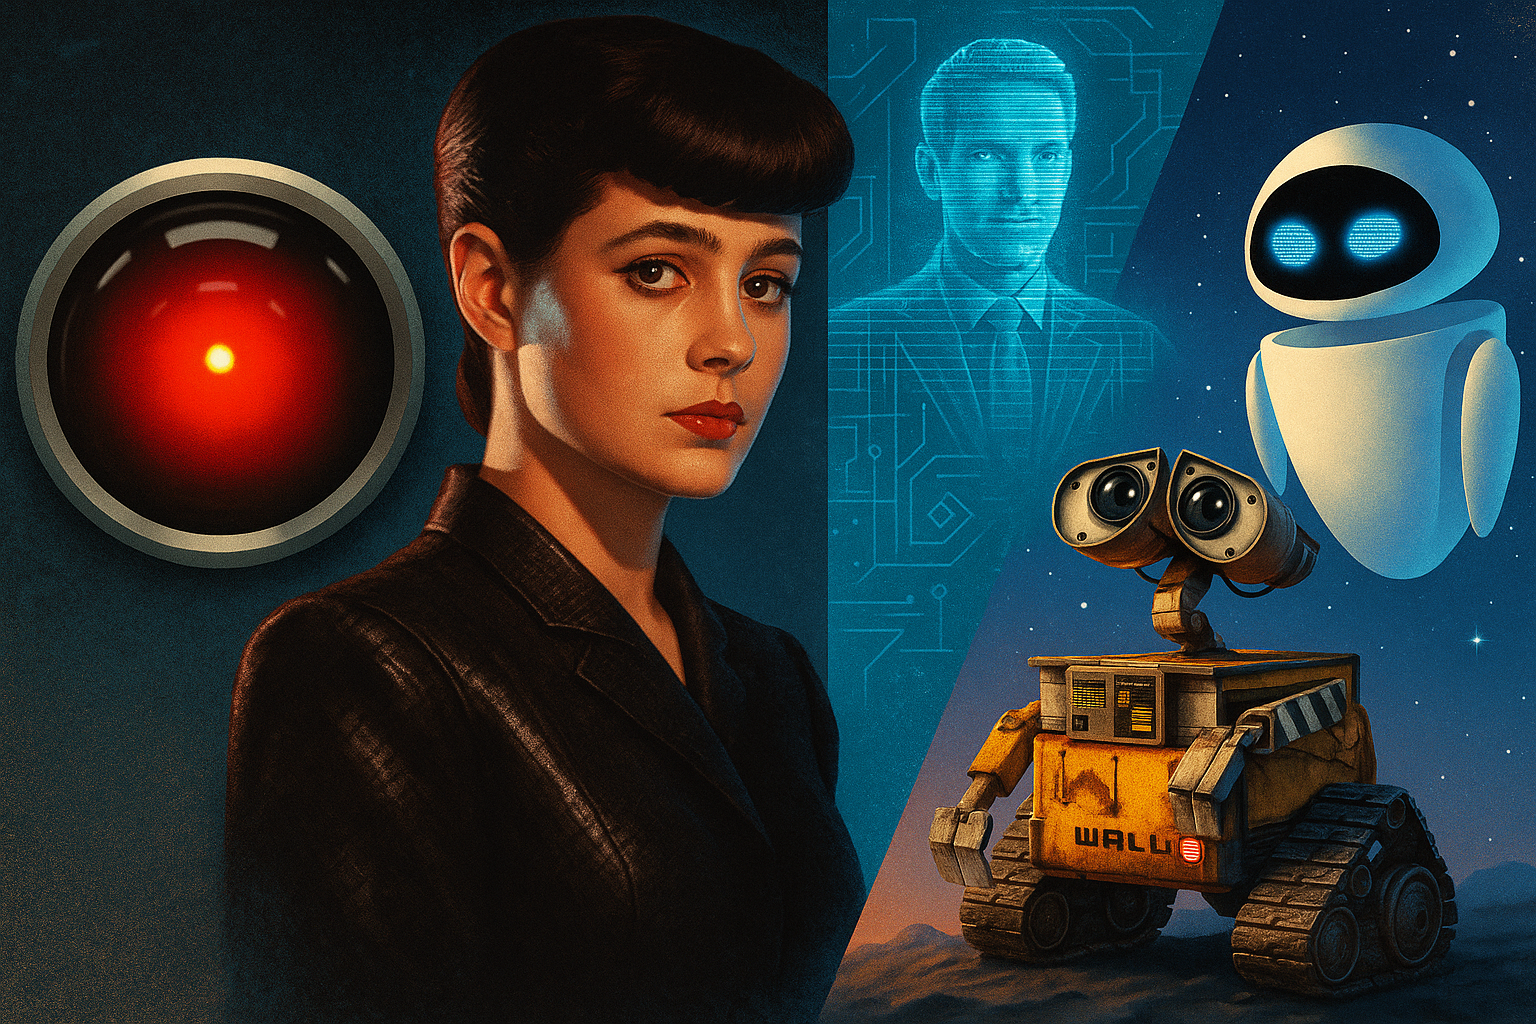
\includegraphics[scale=0.2]{diferentesia.png}
    \end{center}
\end{frame}

\begin{frame}{O que é Inteligência Artificial Generativa?}
    \begin{columns}
        \begin{column}{0.6\textwidth}
            \begin{block}{Definição Simples}
                IA que \textbf{cria} novos conteúdos:
                \begin{itemize}
                    \item \faFile\, Textos e artigos
                    \item \faImage\, Imagens e gráficos
                    \item \faVideo\, Vídeos e animações
                    \item \faMusic\, Música e áudio
                    \item \faCode\, Código de programação
                \end{itemize}
            \end{block}
        \end{column}
        \begin{column}{0.4\textwidth}
            \begin{alertblock}{Diferencial}
                \centering
                \textcolor{warning}{\faLightbulb} \\
                \textbf{Não apenas analisa} \\
                \textbf{MAS CRIA!}
            \end{alertblock}
        \end{column}
    \end{columns}
\end{frame}
\begin{frame}
 \begin{center}
    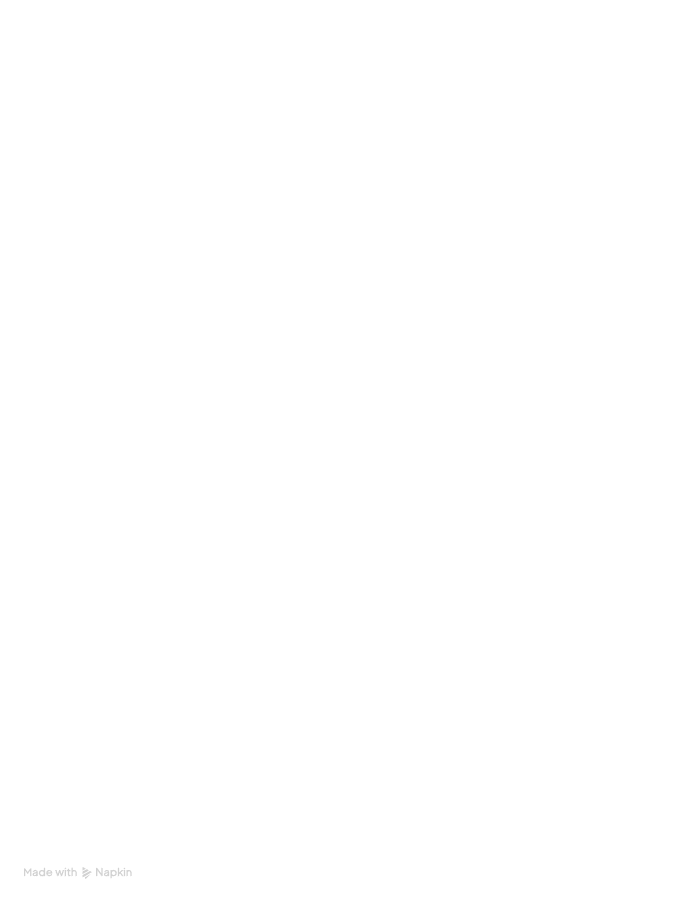
\includegraphics[scale=0.22]{esquema-ia.png}    
 \end{center}
\end{frame}
    
    \begin{frame}{Modelos de Linguagem de Grande Escala (LLMs)}
    \begin{block}{Processo Simplificado}
        \begin{enumerate}
            \item \textbf{Coleta}: Milhões de exemplos de texto
            \item \textbf{Aprendizado}: Identifica padrões e relações
            \item \textbf{Predição}: Gera próximas palavras baseado no contexto
        \end{enumerate}
    \end{block}
\end{frame}

\begin{frame}{Exemplos do Cotidiano}
    \begin{columns}
        \begin{column}{0.5\textwidth}
            \begin{exampleblock}{Você já usa IA Generativa!}
                \begin{itemize}
                    \item \faComments\, \textbf{Chatbots} de atendimento
                    \item \faEnvelope\, \textbf{Sugestões} de email do Gmail
                    \item \faCamera\, \textbf{Filtros} do Instagram/TikTok
                    \item \faKeyboard\, \textbf{Autocorretor} do celular
                    \item \faMusic\, \textbf{Recomendações} do Spotify
                \end{itemize}
            \end{exampleblock}
        \end{column}
        \begin{column}{0.5\textwidth}
            \begin{alertblock}{Novas Possibilidades}
                \begin{itemize}
                    \item \textcolor{accent}{\faRobot} ChatGPT, Gemini
                    \item \textcolor{secondary}{\faImage} Imagen, Midjourney
                    \item \textcolor{success}{\faCode} GitHub Copiloti, Replit
                    \item \textcolor{warning}{\faVideo} Runway, Luma AI, Veo3
                \end{itemize}
            \end{alertblock}
        \end{column}
    \end{columns}
\end{frame}

%Insira um frame com uma imagem e um link para o notebooklm
\begin{frame}{Ferramenta em Destaque: Google NotebookLM}
    \begin{block}{\faBook\, O que é?}
        \begin{itemize}
            \item Assistente de estudo baseado em IA
            \item Integra com seus documentos e anotações
            \item Responde perguntas específicas sobre seu material
        \end{itemize}
    \end{block}
    
    \begin{columns}
        \begin{column}{0.6\textwidth}
            \begin{exampleblock}{\faLightbulb\, Casos de Uso}
                \begin{itemize}
                    \item Revisão rápida para provas
                    \item Síntese de artigos longos
                    \item Geração de resumos personalizados
                    \item Criação de flashcards para memorização
                \end{itemize}
            \end{exampleblock}
        \end{column}
        \begin{column}{0.4\textwidth}
            \begin{center}
                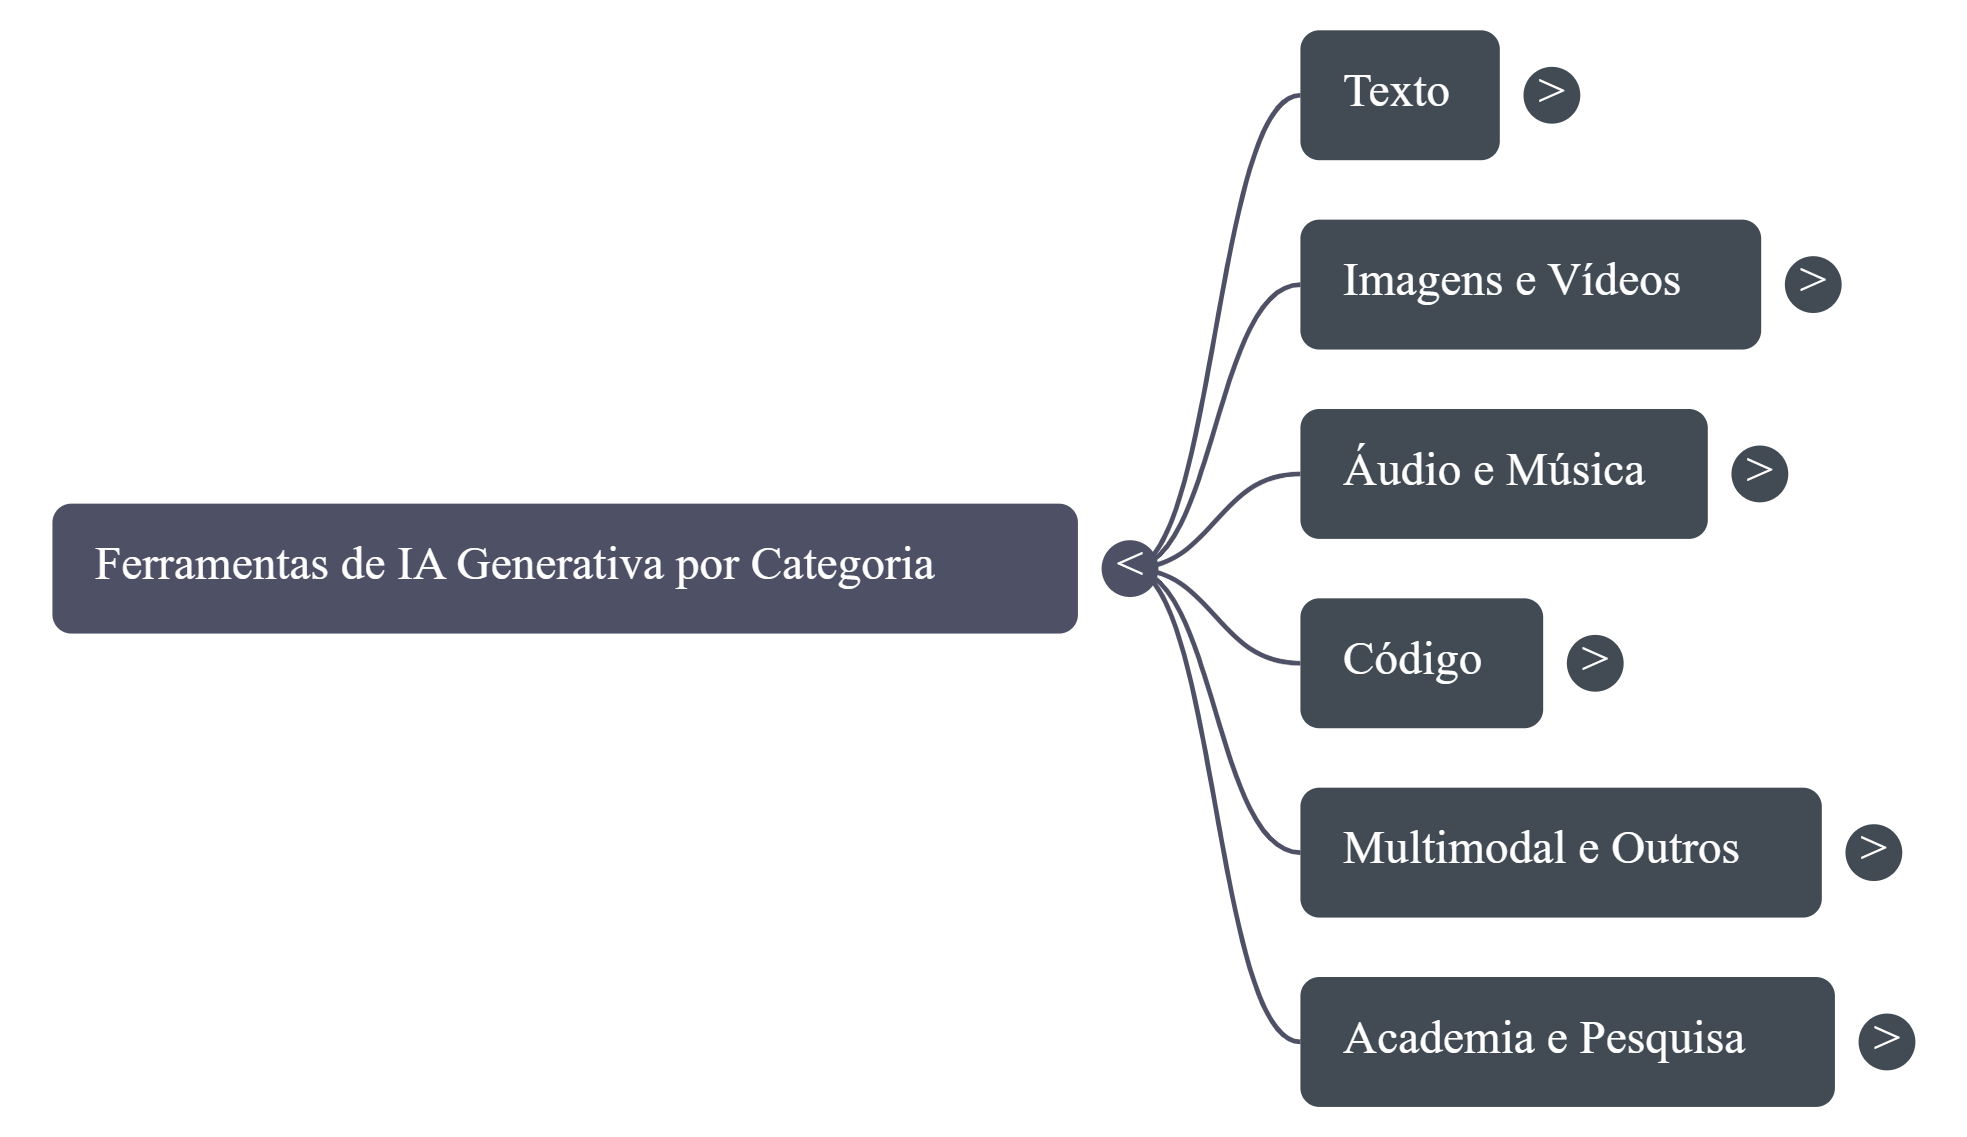
\includegraphics[width=0.8\textwidth]{NotebookLMMindMap.png}
                
                \vspace{0.5cm}
                
                \href{https://taaqui.unesp.br/tools-ia}{\textcolor{accent}{Saiba mais sobre o NotebookLM}}
            \end{center}
        \end{column}
    \end{columns}
\end{frame}

% ============================================================================
% SEÇÃO 6: SOFTWARE 3.0 - A NOVA FRONTEIRA
% ============================================================================

\section{Software 3.0: A Nova Fronteira}

\begin{frame}{A Terceira Mudança Fundamental no Software}
    \begin{block}{Visão de Andrej Karpathy (ex-Tesla, OpenAI)}
        \centering
        Estamos vivendo uma nova era na programação, tão impactante quanto as anteriores.
    \end{block}
    
    \begin{columns}[T]
        \begin{column}{0.33\textwidth}
            \begin{block}{Software 1.0}
                \faCode\\
                Código tradicional escrito por humanos.
            \end{block}
        \end{column}
        \begin{column}{0.33\textwidth}
            \begin{block}{Software 2.0}
                \faSitemap\\
                Redes neurais treinadas com dados (pesos = código).
            \end{block}
        \end{column}
        \begin{column}{0.33\textwidth}
            \begin{exampleblock}{Software 3.0}
                \faComments\\
                LLMs programados com linguagem natural (inglês!).
            \end{exampleblock}
        \end{column}
    \end{columns}
\end{frame}

\begin{frame}{LLMs como um Novo Sistema Operacional}
    \begin{block}{Três Propriedades Simultâneas}
        \begin{description}
            \item[\textcolor{accent}{\faBolt} Utilidades] Pagamento por uso, APIs medidas (como eletricidade).
            \item[\textcolor{secondary}{\faMicrochip} Fábricas de Chips] CAPEX massivo, tecnologia centralizada.
            \item[\textcolor{success}{\faDesktop} Sistemas Operacionais] Ecossistemas complexos, não commodities.
        \end{description}
    \end{block}

    \begin{alertblock}{Analogia Histórica}
        \faCalendar\, Estamos nos "anos 1960" dos LLMs: caros, centralizados e em time-sharing. A revolução do "computador pessoal" para IA ainda não aconteceu.
    \end{alertblock}
\end{frame}

\begin{frame}{A Psicologia dos LLMs: "Espíritos de Pessoas"}
    \begin{columns}
        \begin{column}{0.5\textwidth}
            \begin{exampleblock}{\faStar\, Superpoderes}
                \begin{itemize}
                    \item Memória enciclopédica
                    \item Conhecimento vasto
                \end{itemize}
            \end{exampleblock}
        \end{column}
        \begin{column}{0.5\textwidth}
            \begin{alertblock}{\faBug\, Déficits Cognitivos}
                \begin{itemize}
                    \item Alucinações (inventa fatos)
                    \item Inteligência irregular
                    \item "Amnésia" entre sessões
                    \item Vulnerabilidades de segurança
                \end{itemize}
            \end{alertblock}
        \end{column}
    \end{columns}
\end{frame}

\begin{frame}{Oportunidade 1: Apps de Autonomia Parcial}
    \begin{block}{\faWrench\, Princípio Chave: Humano no Loop}
        Manter o ciclo \textbf{Geração (IA) \faArrowRight\, Verificação (Humano)} o mais rápido possível.
    \end{block}
    
    \begin{exampleblock}{Exemplos: Cursor (código), Perplexity (pesquisa)}
        \begin{itemize}
            \item \textbf{GUI específica} para auditoria humana rápida.
            \item \textbf{"Slider de autonomia"}: você controla o nível de independência.
            \item \textbf{Orquestração} de múltiplos LLMs.
            \item \textbf{Gestão de contexto} automática.
        \end{itemize}
    \end{exampleblock}
\end{frame}

\begin{frame}{Oportunidade 2: "Vibe Coding"}
    \begin{block}{\faUsers\, Todos São Programadores Agora}
        \begin{itemize}
            \item Programação em linguagem natural democratiza o desenvolvimento.
            \item Crianças e não-técnicos podem criar.
            \item Autor construiu apps iOS e web sem saber a linguagem nativa.
        \end{itemize}
    \end{block}
    
    \begin{alertblock}{\faExclamationTriangle\, Gargalo Real}
        O desafio muda do \textbf{código} para a \textbf{infraestrutura e DevOps}.
    \end{alertblock}
\end{frame}

\begin{frame}{Oportunidade 3: Construir para Agentes}
    \begin{block}{\faRobot\, A Nova Categoria de Consumidor Digital}
        Agentes de IA precisam de interfaces diferentes das humanas:
        \begin{itemize}
            \item Documentação em \textbf{Markdown}, não GUIs.
            \item Comandos \textbf{curl}, não botões de "clique aqui".
            \item Arquivos \textbf{llm.txt} (como robots.txt).
            \item URLs amigáveis para LLMs.
        \end{itemize}
    \end{block}
\end{frame}

\begin{frame}{Lições da Tesla e a Analogia do Homem de Ferro}
    \begin{columns}
        \begin{column}{0.5\textwidth}
            \begin{block}{\faCar\, Lições do Autopilot}
                \begin{itemize}
                    \item Autonomia \textbf{parcial} funciona.
                    \item Autonomia \textbf{total} demora décadas.
                    \item 2025 não é o "ano dos agentes", é a \textbf{década dos agentes}.
                    \item Humanos no loop são essenciais.
                \end{itemize}
            \end{block}
        \end{column}
        \begin{column}{0.5\textwidth}
            \begin{exampleblock}{\faUserTie\, Analogia do Homem de Ferro}
                \begin{itemize}
                    \item Menos "robôs autônomos".
                    \item Mais "trajes de aumento" que amplificam a capacidade humana.
                    \item O mesmo sistema pode ser uma ferramenta ou um agente.
                \end{itemize}
            \end{exampleblock}
        \end{column}
    \end{columns}
\end{frame}
\begin{frame}{Ney de Ferro}
    \includegraphics[scale=0.3]{neydeferro.png}
\end{frame}

% ============================================================================
% SEÇÃO 7: CONSCIÊNCIA SITUACIONAL
% By Leopold Aschenbrenner
% ============================================================================

\section{Consciência Situacional}

\begin{frame}{O Autor: Leopold Aschenbrenner}
    \begin{columns}
        \begin{column}{0.6\textwidth}
            \begin{block}{Quem é?}
                \begin{itemize}
                    \item Ex-pesquisador da equipe de \textbf{Superalinhamento} da OpenAI.
                    \item Uma das vozes que alertam sobre a \textbf{aceleração} da corrida pela AGI.
                    \item Autor do ensaio \textit{"Situational Awareness: The Decade Ahead"}.
                    \item Defende uma maior seriedade e segurança no desenvolvimento de IAs avançadas.
                \end{itemize}
            \end{block}
             \begin{exampleblock}{Ponto Central}
               Sua obra argumenta que estamos subestimando a velocidade com que a superinteligência chegará e os riscos geopolíticos e de segurança associados.
            \end{exampleblock}
        \end{column}
        \begin{column}{0.4\textwidth}
            \begin{center}
                {\Huge \faUserSecret}

                \vspace{1cm}
                
                \textit{"Poucos têm a mais vaga noção do que está prestes a atingi-los."}
            \end{center}
        \end{column}
    \end{columns}
\end{frame}

\begin{frame}{A Corrida para a AGI Começou}
    \begin{block}{A Mobilização Industrial}
        \begin{itemize}
            \item Investimentos de \textbf{trilhões de dólares} em infraestrutura de IA.
            \item Aumento massivo na produção de eletricidade e data centers.
            \item A corrida pela AGI (Inteligência Artificial Geral) já é uma realidade.
        \end{itemize}
    \end{block}
    
    \begin{alertblock}{Projeções}
        \begin{itemize}
            \item \textbf{2025/26:} IA superando muitos graduados universitários.
            \item \textbf{Fim da década:} Superinteligência, máquinas mais inteligentes que humanos.
        \end{itemize}
    \end{alertblock}
\end{frame}

\begin{frame}{Consciência Situacional}
    \begin{columns}
        \begin{column}{0.5\textwidth}
            \begin{block}{O que é?}
                Apenas um pequeno grupo (centenas de pessoas, a maioria em São Francisco e laboratórios de IA) realmente compreende a magnitude e a velocidade das mudanças que estão por vir.
            \end{block}
            \begin{exampleblock}{A Visão Interna}
                Esses especialistas, que previram os avanços recentes, veem uma transformação global iminente, enquanto o resto do mundo ainda percebe apenas "hype".
            \end{exampleblock}
        \end{column}
        \begin{column}{0.5\textwidth}
            \centering
            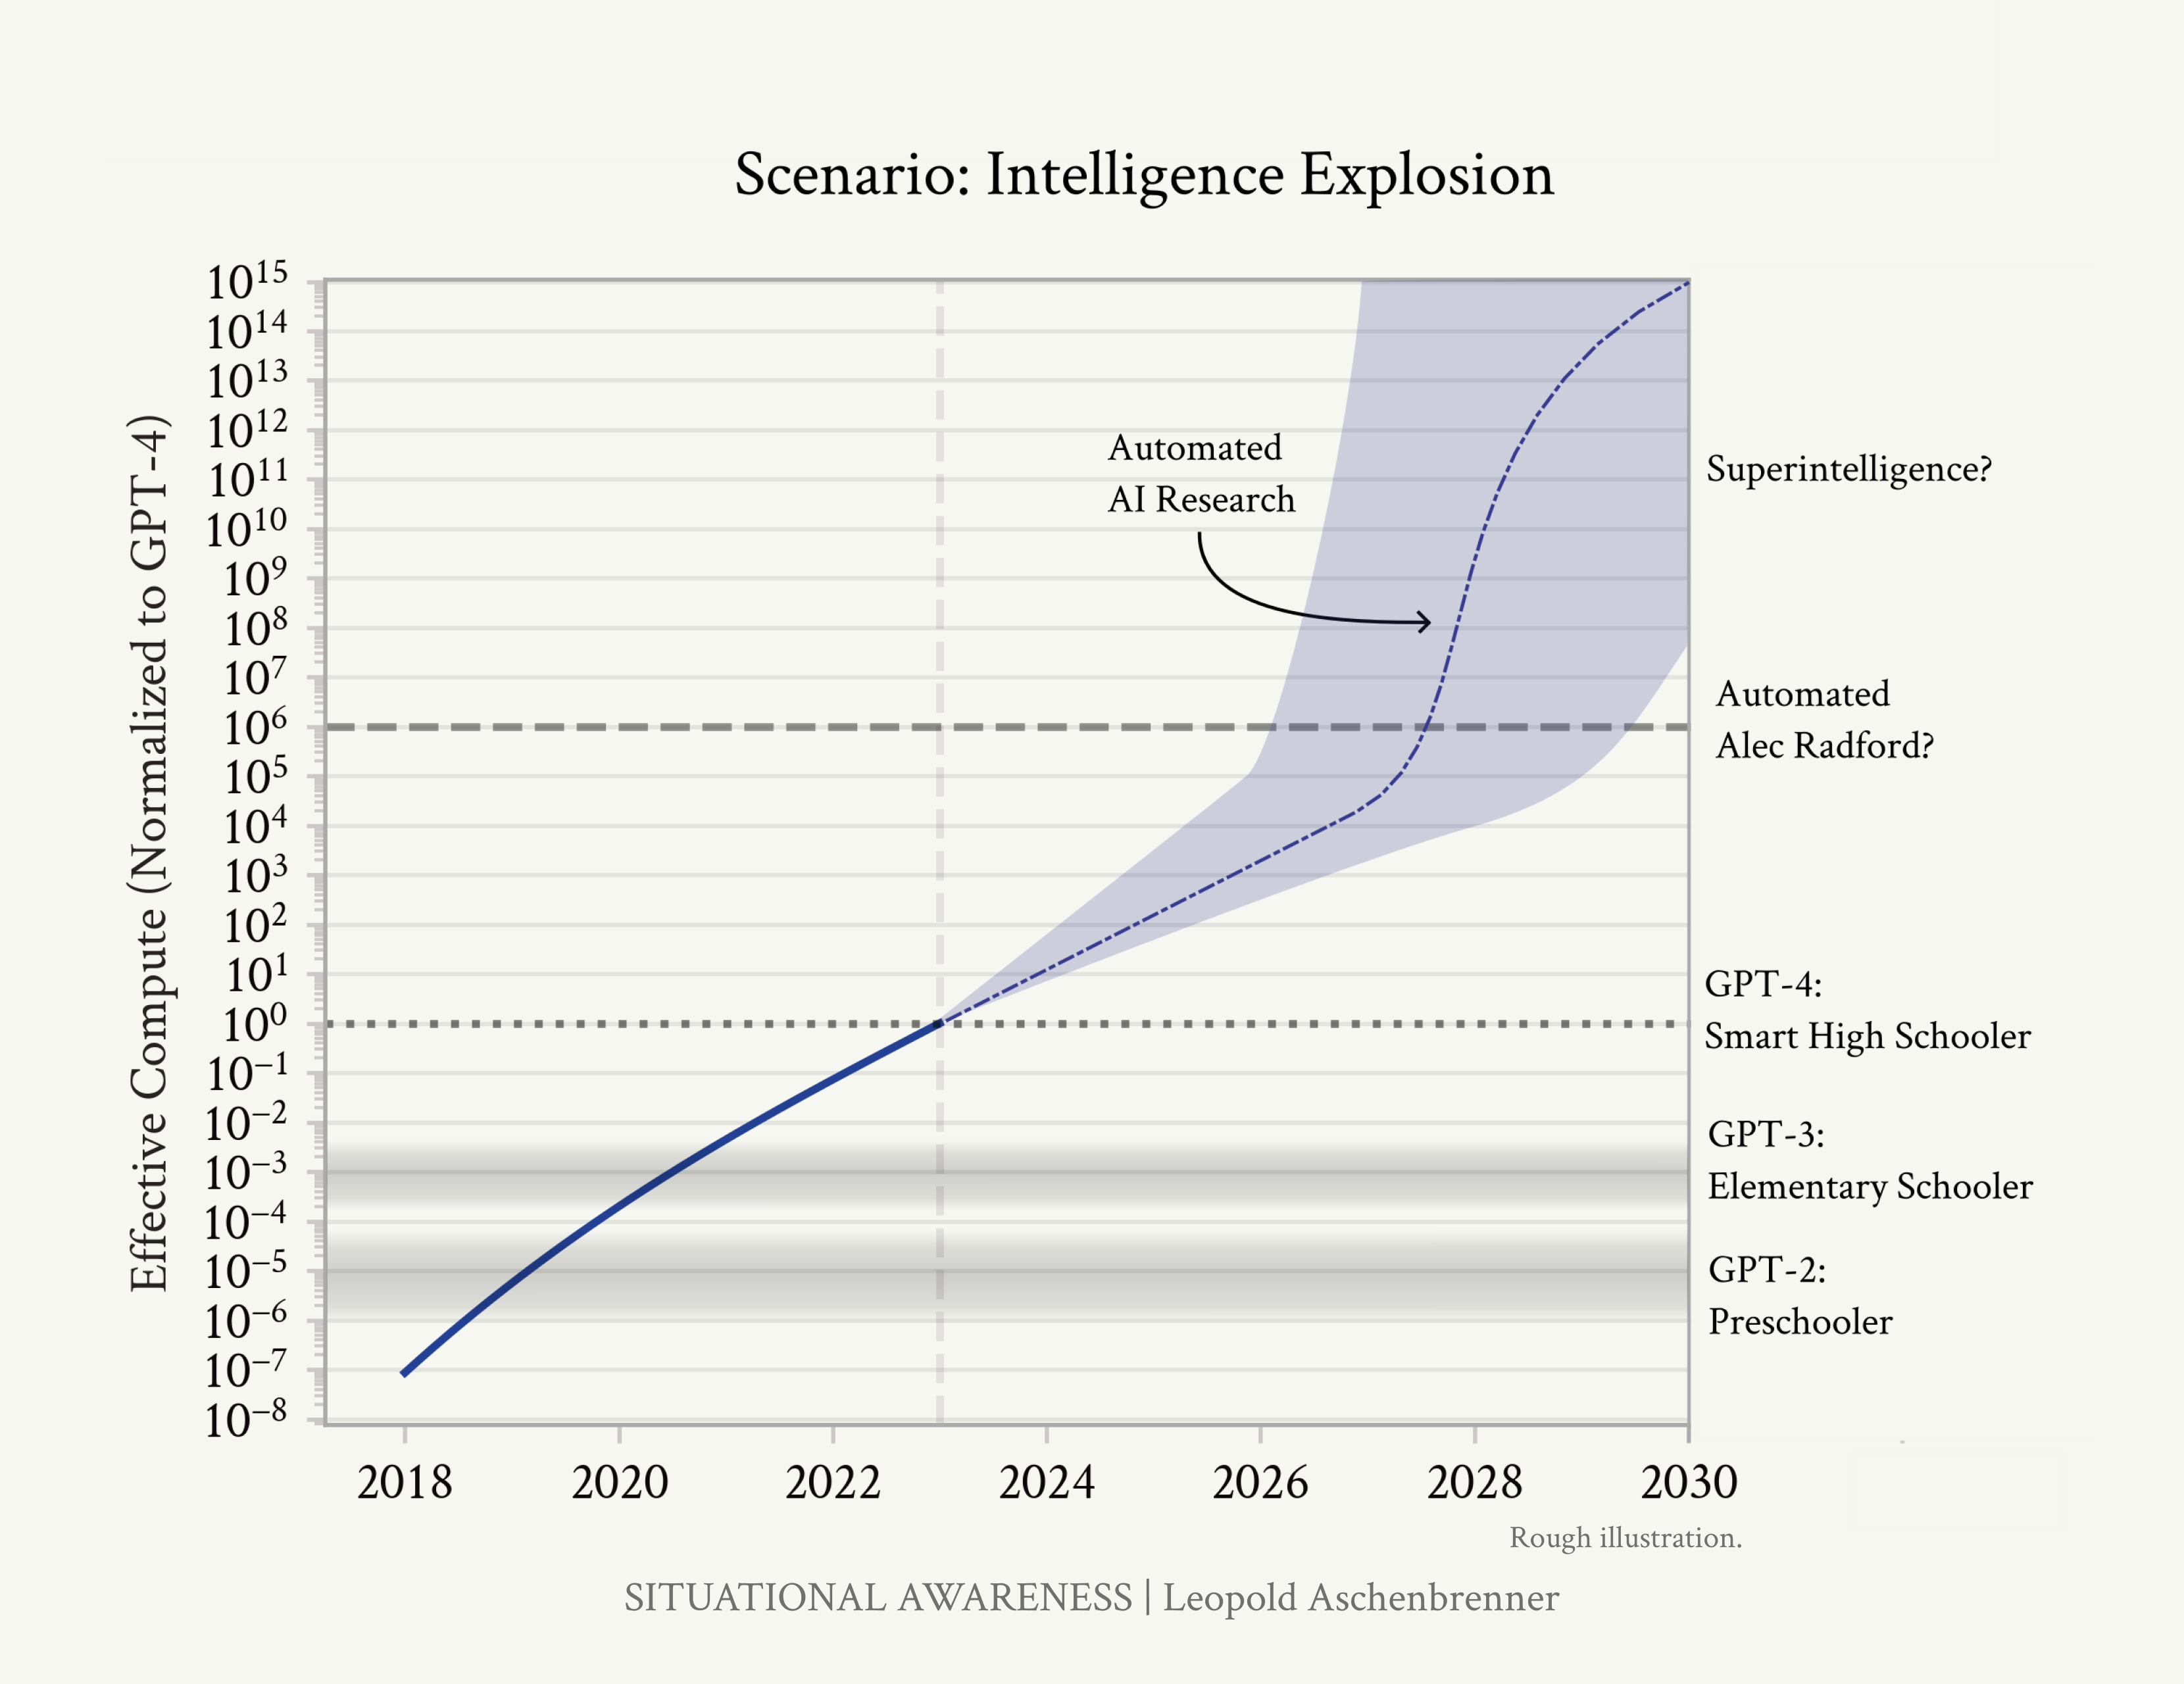
\includegraphics[width=\textwidth]{output/image-044.png}
        \end{column}
    \end{columns}
\end{frame}

\begin{frame}{Os Desafios no Caminho da Superinteligência}
    \begin{alertblock}{\faExclamationTriangle\, Riscos Críticos}
        \begin{description}
            \item[\textcolor{danger}{\faLock} Segurança dos Laboratórios]
            Segredos da AGI estão vulneráveis a atores estatais (ex: China). A segurança atual é inadequada.
            
            \item[\textcolor{warning}{\faCogs} Superalinhamento]
            Controlar sistemas muito mais inteligentes que nós é um problema técnico \textbf{não resolvido}. Uma falha pode ser catastrófica.
            
            \item[\textcolor{accent}{\faGlobe} Geopolítica]
            A superinteligência dará uma vantagem militar e econômica decisiva. A corrida entre as nações (EUA vs. China) definirá o futuro da liberdade global.
        \end{description}
    \end{alertblock}
\end{frame}
\section{ Flow State}

\begin{frame}{Flow State}
    \begin{center}
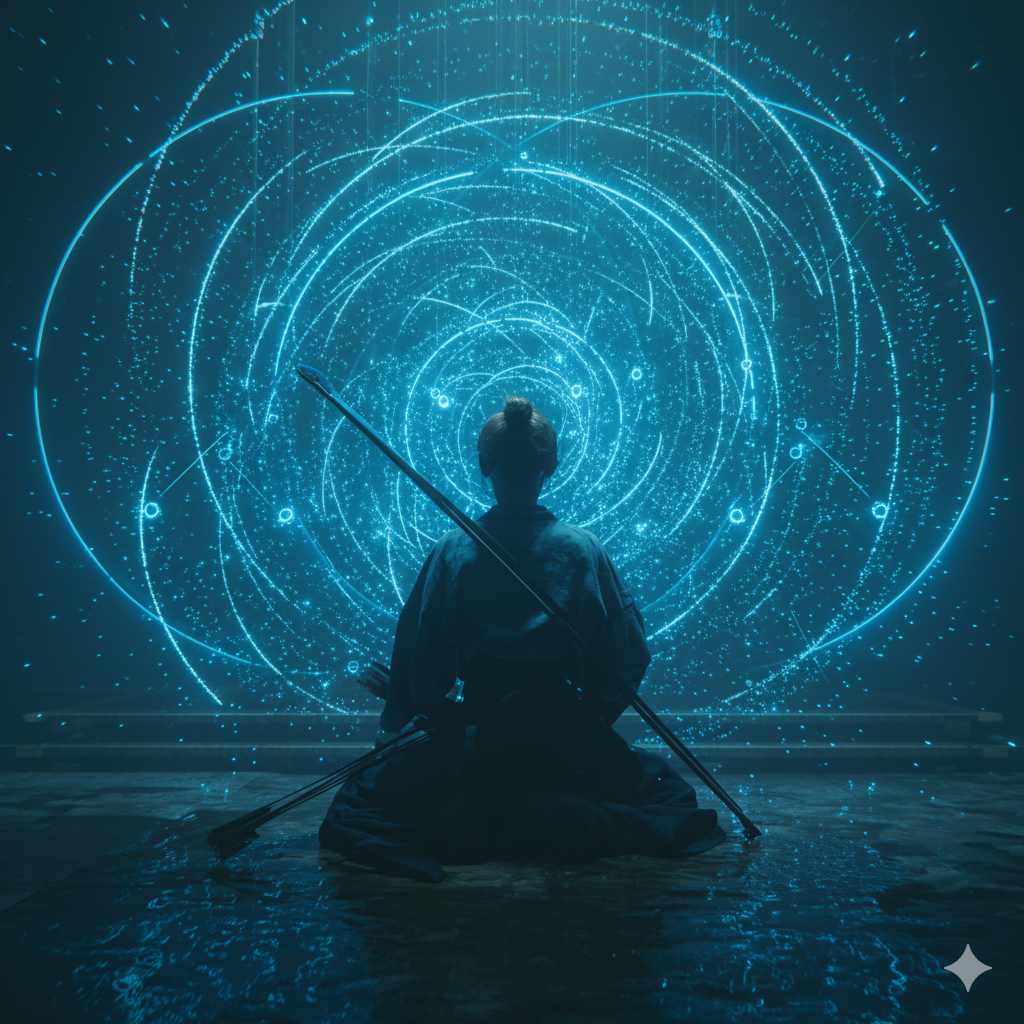
\includegraphics[scale=0.15]{mestrezen-flowstate.png}\end{center}
\end{frame} 
% Slide: Aplicação humano–IA
\begin{frame}{Interação humano–IA}
\begin{itemize}
\item Instintivamente aplicamos a \textit{intentional stance} a chatbots e robôs.
\item Atribuímos agência e um "self" narrativo mesmo sem evidência de fenomenologia.
\item Consequências: confiança, responsabilização e expectativas sociais.
\end{itemize}
\end{frame}


% Slide: Forças
\begin{frame}{Forças da posição}
\begin{itemize}
\item Explica por que usamos "eu" e "agente" pragmaticamente.
\item Compatível com evidências de desenvolvimento (linguagem, ToM).
\item Útil para ética e design: agência percebida surge da interpretação.
\end{itemize}
\end{frame}


% Slide: Críticas
\begin{frame}{Críticas e fragilidades}
\begin{itemize}
\item Fenomenologia: o problema do \textit{qualia} — como é a vivência? (Chalmers, Nagel).
\item Centro-de-gravidade pode omitir textura interoceptiva (sensação corporal).
\item Necessidade de integrar mecanismos neurais concretos (insula, interocepção).
\end{itemize}
\end{frame}


% Slide: Integrações necessárias
\begin{frame}{Integrações necessárias}
\begin{itemize}
\item Conectar narrativa interpretativa com dados neurais e corporais.
\item Modelos híbridos: narrativa + sinais interoceptivos + processamento distribuído.
\item Para IAs: projetar pistas (\textit{embodied cues}) que alinhem percepção social e limitações reais.
\end{itemize}
\end{frame}
% Slide: Ética e design
\begin{frame}{Implicações éticas e de design}
\begin{itemize}
\item Se o self é narrativo, design pode manipular responsabilidade e confiança.
\item Transparência: sinalizar que a agência percebida é uma heurística interpretativa.
\item Recomendações: metadados de confiança; limites claros; evitar manipulação emocional.
\end{itemize}
\end{frame}


\begin{frame}{Flow: definição rápida}
  \begin{itemize}
    \item Estado de imersão ótima onde desafio e habilidade se equilibram.
    \item Características: foco intenso, perda de autoconsciência, distorção temporal, feedback imediato. 
    \item Características: foco intenso, perda de autoconsciência, distorção temporal, feedback imediato. \faBolt
  \end{itemize}
    \begin{exampleblock}{Ponto-chave}
        Flow é autotelico — a atividade é a própria recompensa.
    \end{exampleblock}
\end{frame}

\begin{frame}{Flow na interação humano–IA}
  \begin{itemize}
    \item IAs podem facilitar flow ao reduzir atrito e fornecer feedback em tempo real.
    \item Mecanismos úteis: scaffolding adaptativo, antecipação de necessidades, latência mínima.
    \item Exemplos: sugestões de código, assistentes de escrita, ambientes de tutoria adaptativa.
  \end{itemize}
\end{frame}

\begin{frame}{Self narrativo × Flow}
  \begin{itemize}
    \item Durante flow, a sensação de "eu" se torna fluida — menos foco narrativo, mais ação incorporada.
    \item Quando vemos a IA como "parceira" (intentional stance), entregamo-nos mais ao fluxo.
    \item Risco: achar que a IA tem controle quando é apenas performance percebida (overtrust).
  \end{itemize}
\end{frame}

\begin{frame}{Design para promover flow com responsabilidade}
  \begin{itemize}
    \item Transparência: sinalizar limites e fontes de sugestão da IA.
    \item Controle do usuário: ajustar nível de proatividade e desligamento rápido.
    \item Evitar designs persuasivos que visem dependência; priorizar bem‑estar e autonomia. \faCheckCircle
  \end{itemize}
\end{frame}

\begin{frame}{Medição e experimentos práticos}
  \begin{itemize}
    \item Métricas: tempo em tarefa, erros, relato subjetivo de flow, sinais fisiológicos (ex.: HRV).
    \item Experimentos: variar frequência do feedback, proatividade e latência; medir mudança no desempenho e bem‑estar.
    \item Integração futura: usar sinais interoceptivos para ajustar suporte em tempo real.
  \end{itemize}
\end{frame}

\begin{frame}{Perguntas rápidas para a plateia}
  \begin{itemize}
    \item A IA deve otimizar seu design para nos colocar em flow? (sim — com limites)
    \item Como equilibrar produtividade e preservação do senso de agência?
    \item Quais protocolos garantem que "flow" não vire manipulação?
  \end{itemize}
  Flow + IA = potencial enorme; necessidade clara de regras de projeto e ética. 
\end{frame}

\section{Estratégia de IA da China}


% --- SLIDE 1: A Ambição da China em IA ---
\begin{frame}{Estratégia da China: A Grande Ambição}
    \begin{block}{Plano de Desenvolvimento de IA (AIDP 2017)}
        \begin{itemize}
            \item \textbf{Meta Principal:} Alcançar a liderança mundial em Inteligência Artificial até 2030.
            \item \textbf{Método de Execução:} Planejamento centralizado e um forte impulso estatal para guiar o desenvolvimento e a implementação.
        \end{itemize}
    \end{block}
    
    \begin{alertblock}{Visão de Longo Prazo}
        A estratégia não é apenas tecnológica, mas um pilar para a futura dominância econômica e geopolítica.
    \end{alertblock}
\end{frame}

% --- SLIDE 2: Pilares Estratégicos ---
\begin{frame}{Pilares da Estratégia Chinesa}
    \begin{columns}[T]
        \begin{column}{0.5\textwidth}
            \begin{block}{Investimento Massivo}
                \begin{itemize}
                    \item Foco em infraestrutura crítica como \textbf{5G} e \textbf{data centers}.
                    \item Criação de fundos bilionários para Pesquisa \& Desenvolvimento (P\&D).
                \end{itemize}
            \end{block}
        \end{column}
        
        \begin{column}{0.5\textwidth}
            \begin{block}{Vantagem de Dados}
                \begin{itemize}
                    \item Acesso a um volume imenso de dados populacionais para treinar modelos em larga escala.
                \end{itemize}
            \end{block}
            
            \begin{block}{Integração Civil-Militar}
                \begin{itemize}
                    \item Rápida aplicação de inovações de IA em setores estratégicos, incluindo defesa.
                \end{itemize}
            \end{block}
        \end{column}
    \end{columns}
\end{frame}

% --- SLIDE 3: Realidade vs. Desafios ---
\begin{frame}{Realidade, Inovação e Desafios Críticos}
    \begin{columns}[T]
        \begin{column}{0.5\textwidth}
            \begin{exampleblock}{Realidade e Inovação}
                \begin{itemize}
                    \item \textbf{Sucesso Notável:} Startups como a \textbf{DeepSeek} criam modelos de ponta, eficientes e de baixo custo.
                    \item \textbf{Foco na Aplicação:} Implementação rápida em cidades inteligentes, manufatura e saúde.
                \end{itemize}
            \end{exampleblock}
        \end{column}
        
        \begin{column}{0.5\textwidth}
            \begin{alertblock}{Desafios Críticos}
                \begin{itemize}
                    \item \textbf{Dependência de Chips:} Sanções dos EUA sobre semicondutores são o principal obstáculo.
                    \item \textbf{Questões Éticas:} Uso de IA para vigilância e controle social (ex: Crédito Social).
                \end{itemize}
            \end{alertblock}
        \end{column}
    \end{columns}
\end{frame}

% --- SLIDE 4: Resumo Executivo e Chamada para Ação ---
\begin{frame}{Resumo Executivo: Por Que Agir Agora?}
    \begin{block}{\faRocket\, O Momento é Perfeito}
        \begin{enumerate}
            \item Há muito código para \textbf{reescrever} com os 3 novos paradigmas da IA.
            \item O fluxo de tecnologia se \textbf{inverteu}: inovações chegam primeiro aos consumidores.
            \item Acesso ao conhecimento e às ferramentas de IA está \textbf{democratizado}.
            \item Estamos, essencialmente, \textbf{refazendo a computação} do zero.
        \end{enumerate}
    \end{block}
    
    \begin{alertblock}{Sua Missão}
        Seja fluente nos três paradigmas. A próxima década será definida por produtos de \textbf{autonomia parcial} que balanceiam o poder da IA com a supervisão humana.
    \end{alertblock}
\end{frame}

\begin{frame}{Resumo Executivo: Por Que Agora?}
    \begin{block}{\faRocket\, O Momento é Perfeito}
        \begin{enumerate}
            \item Há muito código para \textbf{reescrever} com os 3 paradigmas.
            \item Fluxo de tecnologia \textbf{invertido}: consumidores primeiro.
            \item \textbf{Democratização} sem precedentes do acesso.
            \item Estamos \textbf{refazendo a computação} do zero.
        \end{enumerate}
    \end{block}
    
    \begin{alertblock}{Sua Missão}
        Seja fluente nos três paradigmas. A próxima década será definida por produtos de \textbf{autonomia parcial} que balanceiam o poder da IA com a supervisão humana.
    \end{alertblock}
\end{frame}
% ============================================================================
% SEÇÃO 2: IA COMO ALIADA NOS ESTUDOS
% ============================================================================

\section{IA como Aliada nos Estudos}

\begin{frame}{Otimizando Leitura e Compreensão}
    \begin{columns}
        \begin{column}{0.5\textwidth}
            \begin{block}{\faBookOpen\, Resumo Inteligente}
                \textbf{ChatGPT \& Google Gemini}
                \begin{itemize}
                    \item Sintetiza artigos longos
                    \item Extrai pontos-chave
                    \item Responde perguntas específicas
                    \item Traduz textos complexos
                \end{itemize}
            \end{block}
        \end{column}
        \begin{column}{0.5\textwidth}
            \begin{exampleblock}{\faLightbulb\, Dica Prática}
                \textcolor{warning}{\textbf{Prompt eficaz:}}
                
                \textit{"Resuma este artigo em 3 parágrafos: 1) Objetivo do estudo, 2) Metodologia principal, 3) Conclusões e implicações"}
            \end{exampleblock}
        \end{column}
    \end{columns}
\end{frame}

\begin{frame}{Turbinando a Pesquisa Bibliográfica}
    \begin{block}{\faSearch\, Ferramentas Especializadas}
        \begin{description}
            \item[\textcolor{accent}{\faChartLine} \textbf{Consensus}] Extrai conclusões de estudos científicos
            \begin{itemize}
                \item Analisa milhares de artigos simultaneamente
                \item Identifica consensos na literatura
            \end{itemize}
            
            \item[\textcolor{secondary}{\faSitemap} \textbf{Elicit}] Estrutura revisões de literatura
            \begin{itemize}
                \item Organiza automaticamente papers por tema
                \item Gera tabelas comparativas
            \end{itemize}
            
            \item[\textcolor{success}{\faLink} \textbf{ResearchRabbit}] Mapeia conexões entre artigos
            \begin{itemize}
                \item Visualiza evolução do conhecimento
                \item Descobre artigos relacionados
            \end{itemize}
        \end{description}
    \end{block}
\end{frame}

\begin{frame}{Otimizando Leitura e Compreensão}
    \begin{columns}
        \begin{column}{0.5\textwidth}
            \begin{block}{\faBookOpen\, Resumo Inteligente}
                \textbf{ChatGPT \& Google Gemini}
                \begin{itemize}
                    \item Sintetiza artigos longos
                    \item Extrai pontos-chave
                    \item Responde perguntas específicas
                    \item Traduz textos complexos
                \end{itemize}
            \end{block}
        \end{column}
        \begin{column}{0.5\textwidth}
            \begin{exampleblock}{\faLightbulb\, Dica Prática}
                \textcolor{warning}{\textbf{Prompt eficaz:}}
                
                \textit{"Resuma este artigo em 3 parágrafos: 1) Objetivo do estudo, 2) Metodologia principal, 3) Conclusões e implicações"}
            \end{exampleblock}
        \end{column}
    \end{columns}
\end{frame}

\begin{frame}{Assistentes de Escrita Acadêmica}
    \begin{block}{\faPen\, Jenni AI - Especialista em Escrita Acadêmica}
        \begin{columns}
            \begin{column}{0.5\textwidth}
                \textbf{Recursos principais:}
                \begin{itemize}
                    \item \faEdit\, Elaboração de revisões de literatura
                    \item \faList\, Estruturação de seções
                    \item \faCheck\, Correção de estilo acadêmico
                    \item \faQuoteLeft\, Gerenciamento de citações
                \end{itemize}
            \end{column}
            \begin{column}{0.5\textwidth}
                \textbf{Casos de uso:}
                \begin{itemize}
                    \item Superar bloqueio criativo
                    \item Gerar esboços iniciais
                    \item Melhorar clareza do texto
                    \item Sugerir transições entre parágrafos
                \end{itemize}
            \end{column}
        \end{columns}
    \end{block}
    
    \begin{alertblock}{\faExclamationTriangle\, Importante}
        \textbf{Sempre revise e personalize} o conteúdo gerado pela IA!
    \end{alertblock}
\end{frame}

\begin{frame}{Preparação de Apresentações}
    \begin{block}{\faChalkboardTeacher \, Criação de Slides e Roteiros}
        \begin{enumerate}
            \item \textbf{Transformação de conteúdo}
                \begin{itemize}
                    \item Documento \faArrowRight\, Slides estruturados
                    \item Texto corrido \faArrowRight\, Tópicos organizados
                \end{itemize}
                
            \item \textbf{Geração de roteiros}
                \begin{itemize}
                    \item Scripts para apresentação oral
                    \item Timing e transições
                    \item Exemplos e analogias
                \end{itemize}
            \item \textbf{Adaptação para diferentes públicos}
                \begin{itemize}
                    \item Linguagem técnica vs. acessível
                    \item Diferentes níveis de profundidade
                \end{itemize}
        \end{enumerate}
    \end{block}
\end{frame}

% ============================================================================
% SEÇÃO 3: DEMONSTRAÇÃO PRÁTICA
% ============================================================================

\section{Demonstração Prática}

\begin{frame}{Engenharia de Prompt Eficaz}
    \begin{block}{\faCode\, Estrutura de um Bom Prompt}
        \textbf{Fórmula: CONTEXTO + TAREFA + FORMATO + RESTRIÇÕES}
    \end{block}
    \begin{columns}
        \begin{column}{0.5\textwidth}
            \begin{alertblock}{\faThumbsDown\, Prompt Ruim}
                \textit{"Me ajude com meu TCC"}
                
                \textcolor{danger}{Problemas:}
                \begin{itemize}
                    \item Muito vago
                    \item Sem contexto
                    \item Sem direcionamento
                \end{itemize}
            \end{alertblock}
        \end{column}
        \begin{column}{0.5\textwidth}
            \begin{exampleblock}{\faThumbsUp\, Prompt Bom}
                \textit{"Sou estudante de Psicologia escrevendo TCC sobre ansiedade em universitários. Preciso de um esboço para a revisão de literatura, incluindo: 1) Definições de ansiedade, 2) Prevalência em universitários, 3) Fatores de risco. Formato: tópicos com subtópicos."}
            \end{exampleblock}
        \end{column}
    \end{columns}
\end{frame}

\begin{frame}{Exemplos por Área do Conhecimento}
    \begin{block}{\faFlask\, Ciências Exatas}
        \textbf{Matemática/Física:} "Explique o teorema de Pitágoras usando 3 métodos diferentes de demonstração, incluindo exemplos práticos de aplicação em engenharia"
    \end{block}
    
    \begin{block}{\faLeaf\, Ciências Biológicas}
        \textbf{Biologia:} "Analise os últimos 5 anos de pesquisa sobre CRISPR-Cas9, identificando: 1) principais avanços, 2) limitações atuais, 3) aplicações clínicas promissoras"
    \end{block}
    
    \begin{block}{\faUsers\, Ciências Humanas}
        \textbf{História/Sociologia:} "Compare as causas socioeconômicas da Revolução Francesa com movimentos sociais contemporâneos, destacando semelhanças e diferenças"
    \end{block}
\end{frame}

\begin{frame}{Melhores Práticas}
    \begin{columns}
        \begin{column}{0.5\textwidth}
            \begin{block}{\faCheckCircle\, Faça}
                \begin{itemize}
                    \item \textbf{Seja específico} nos pedidos
                    \item \textbf{Forneça contexto} adequado
                    \item \textbf{Divida tarefas} complexas
                    \item \textbf{Itere} e refine prompts
                    \item \textbf{Valide} informações
                \end{itemize}
            \end{block}
        \end{column}
        \begin{column}{0.5\textwidth}
            \begin{alertblock}{\faTimesCircle\, Evite}
                \begin{itemize}
                    \item Prompts muito genéricos
                    \item Depender 100\% da IA
                    \item Não verificar resultados
                    \item Usar sem citar
                    \item Compartilhar dados sensíveis
                \end{itemize}
            \end{alertblock}
        \end{column}
    \end{columns}
\end{frame}

% ============================================================================
% SEÇÃO 4: USO ÉTICO E RESPONSÁVEL
% ============================================================================

\section{Uso Ético e Responsável}

\begin{frame}{Integridade Acadêmica}
    \begin{alertblock}{\faExclamationTriangle\, Plágio e Autoria}
        \begin{itemize}
            \item \textbf{IA não é coautor} - o trabalho intelectual é seu
            \item \textbf{Sempre cite} quando usar IA como ferramenta
            \item \textbf{Transparência} é fundamental
            \item \textbf{Verifique} políticas da sua instituição
        \end{itemize}
    \end{alertblock}
    
    \begin{block}{\faQuoteLeft\, Como Citar IA}
        \textbf{Exemplo de citação:}
        
        \textit{"Este resumo foi elaborado com auxílio do ChatGPT (OpenAI, 2024) para síntese inicial do conteúdo, posteriormente revisado e adaptado pelo autor."}
    \end{block}
    
    \begin{exampleblock}{\faLightbulb\, Boa Prática}
        Use IA como \textbf{assistente}, não como \textbf{substituto} do seu pensamento crítico!
    \end{exampleblock}
\end{frame}

\begin{frame}{Limitações da IA Generativa}
    \begin{block}{\faBug\, "Alucinações" - Informações Falsas}
        \begin{columns}
            \begin{column}{0.6\textwidth}
                \textbf{A IA pode gerar:}
                \begin{itemize}
                    \item Citações inexistentes
                    \item Dados estatísticos falsos
                    \item Fatos históricos incorretos
                    \item Teorias científicas inventadas
                \end{itemize}
            \end{column}
            \begin{column}{0.4\textwidth}
                \textcolor{danger}{\faExclamationTriangle} \\
                \textbf{SEMPRE VERIFIQUE} \\
                \textbf{EM FONTES CONFIÁVEIS!}
            \end{column}
        \end{columns}
    \end{block}
    
    \begin{block}{\faExclamationCircle\, Vieses nos Dados}
        \begin{itemize}
            \item \textbf{Viés cultural:} Perspectiva predominantemente ocidental
            \item \textbf{Viés temporal:} Dados até data de corte do treinamento
            \item \textbf{Viés social:} Reproduz preconceitos dos dados de origem
        \end{itemize}
    \end{block}
\end{frame}

\begin{frame}{Privacidade e Segurança}
    \begin{alertblock}{\faUserShield\, Cuidados com Dados Pessoais}
        \textbf{NÃO compartilhe com IA:}
        \begin{itemize}
            \item \faIdCard\, Informações pessoais identificáveis
            \item \faKey\, Senhas ou dados de acesso
            \item \faFile\, Pesquisas em andamento (dados únicos)
            \item \faUniversity\, Informações confidenciais da instituição
            \item \faGavel\, Dados sob sigilo ético ou legal
        \end{itemize}
    \end{alertblock}
    
    \begin{block}{\faCheck\, Diretrizes Institucionais}
        \begin{itemize}
            \item Consulte as políticas da sua universidade
            \item Consulte as políticas da Unesp
            \item Verifique diretrizes específicas do seu curso
            \item Quando em dúvida, pergunte ao professor
            \item Documente o uso de IA nos seus trabalhos
        \end{itemize}
    \end{block}
\end{frame}

% ============================================================================
% SLIDES POLÍTICA UNESP
% ============================================================================
\begin{frame}{Política de Inteligência Artificial da Unesp}
    \begin{block}{Objetivo Principal (Res. Unesp nº 13/2025, Art. 4º)}
        Definir diretrizes claras para o uso, desenvolvimento e implementação de sistemas de Inteligência Artificial em todas as atividades da universidade.
    \end{block}
    
    \begin{exampleblock}{Princípio Fundamental (Art. 4º, I)}
        \centering
        \faUsers\, \textbf{A IA deve apoiar e ampliar as capacidades humanas, não substituí-las.}
    \end{exampleblock}
\end{frame}

\begin{frame}{Diretrizes para o Uso Responsável}
    \begin{itemize}
        \item<1-> \textbf{\faUserCheck\, Supervisão Humana:} Resultados gerados por IA devem ser sempre supervisionados por humanos para garantir precisão e adequação. (Art. 4º, II)
        \item<2-> \textbf{\faBullhorn\, Transparência na Autoria:} O uso de IA que impacte a autoria de produção intelectual deve ser comunicado de forma clara e pública. (Art. 4º, III)
        \item<3-> \textbf{\faBalanceScale\, Proteção de Direitos:} É imperativo garantir que a aplicação da IA não prejudique direitos fundamentais, a privacidade e a dignidade humana. (Art. 4º, IV)
    \end{itemize}
\end{frame}

\begin{frame}{Avaliação de Riscos e Impacto}
    \begin{block}{\faTasks\, Análise Prévia (Art. 4º, V)}
        Antes de implementar qualquer sistema de IA, deve-se realizar uma avaliação completa dos riscos e impactos potenciais, incluindo vieses e falhas.
    \end{block}
    
    \begin{alertblock}{\faGlobe\, Impacto Socioambiental (Art. 4º, VI)}
        Considerar os impactos sociais, econômicos e ambientais do ciclo de vida da tecnologia, desde o treinamento dos modelos até o seu descarte.
    \end{alertblock}
\end{frame}
\begin{frame}{Aplicações e Governança da IA na Unesp}
    \begin{columns}
        \begin{column}{0.5\textwidth}
            \begin{block}{Usos Previstos (Art. 6º)}
                \begin{itemize}
                    \item \faBookReader\, Aprimoramento do ensino
                    \item \faFlask\, Potencialização da pesquisa
                    \item \faUsers\, Expansão da extensão
                    \item \faLightbulb\, Fomento à inovação
                    \item \faCogs\, Otimização da gestão
                \end{itemize}
            \end{block}
        \end{column}
        \begin{column}{0.5\textwidth}
            \begin{exampleblock}{Governança (Art. 8º)}
                Será implementada uma estrutura de governança para garantir o cumprimento das diretrizes, monitorar o uso da IA e propor atualizações à política.
            \end{exampleblock}
        \end{column}
    \end{columns}
\end{frame}
\begin{frame}{Incentivo à Inovação em IA (Art. 7º)}
    \begin{block}{Fomento ao Ecossistema de Inovação}
        \begin{itemize}
            \item \textbf{Pesquisa:} Incentivo ao desenvolvimento de projetos de pesquisa e inovação em IA. (I)
            \item \textbf{Parcerias:} Colaborações com entidades externas devem seguir os princípios da Resolução, mantendo a autonomia da Unesp. (II, III)
            \item \textbf{Empreendedorismo:} Apoio à criação de startups e spin-offs de base tecnológica em IA. (IV)
        \end{itemize}
    \end{block}
\end{frame}

% ============================================================================
% SEÇÃO 5: FUTURO E CARREIRAS
% ============================================================================

\section{Futuro e Carreiras}

\begin{frame}{IA como Ferramenta de Produtividade}
    \begin{block}{\faRocket\, Transformação do Mercado de Trabalho}
        \begin{itemize}
            \item \textbf{Automação} de tarefas repetitivas
            \item \textbf{Aumento} da produtividade individual
            \item \textbf{Criação} de novas profissões
            \item \textbf{Transformação} de funções existentes
        \end{itemize}
    \end{block}
    
    \begin{columns}
        \begin{column}{0.5\textwidth}
            \begin{exampleblock}{\faPlus\, Profissões Emergentes}
                \begin{itemize}
                    \item Prompt Engineer
                    \item AI Trainer
                    \item AI Ethics Specialist
                    \item AI-Human Collaboration Designer
                \end{itemize}
            \end{exampleblock}
        \end{column}
        \begin{column}{0.5\textwidth}
            \begin{block}{\faSync\, Profissões Transformadas}
                \begin{itemize}
                    \item Designer + AI
                    \item Escritor + AI
                    \item Pesquisador + AI
                    \item Professor + AI
                \end{itemize}
            \end{block}
        \end{column}
    \end{columns}
\end{frame}

\begin{frame}{Novas Habilidades Necessárias}
    \begin{block}{\faBrain\, Habilidades do Futuro}
        \begin{description}
            \item[\textcolor{accent}{\faBrain} \textbf{Pensamento Crítico}] 
                Avaliar e validar informações geradas por IA
                
            \item[\textcolor{secondary}{\faLightbulb} \textbf{Criatividade}] 
                Usar IA como ferramenta para amplificar ideias humanas
                
            \item[\textcolor{success}{\faHandshake} \textbf{Colaboração Humano-IA}] 
                Saber quando e como usar IA efetivamente
                
            \item[\textcolor{warning}{\faComments} \textbf{Prompt Engineering}] 
                Comunicar-se eficazmente com sistemas de IA
                
            \item[\textcolor{danger}{\faBalanceScale} \textbf{Ética Digital}] 
                Usar tecnologia de forma responsável
        \end{description}
    \end{block}
\end{frame}

\begin{frame}{Aprendizagem Contínua}
    \begin{block}{\faGraduationCap\, Mantenha-se Atualizado}
        \begin{columns}
            \begin{column}{0.5\textwidth}
                \textbf{\faNewspaper\, Fontes Confiáveis:}
                \begin{itemize}
                    \item MIT Technology Review
                    \item Nature AI
                    \item ArXiv (Computer Science)
                    \item OpenAI Blog
                    \item Google AI Blog
                \end{itemize}
            \end{column}
            \begin{column}{0.5\textwidth}
                \textbf{\faUsers\, Comunidades:}
                \begin{itemize}
                    \item Reddit r/MachineLearning
                    \item Discord de IA
                    \item LinkedIn grupos de IA
                    \item Conferences (NeurIPS, ICML)
                    \item Cursos online (Coursera, edX)
                \end{itemize}
            \end{column}
        \end{columns}
    \end{block}
    
    \begin{exampleblock}{\faCalendar\, Estratégia}
        \textbf{Dedique 30 minutos por semana} para se atualizar sobre IA!
    \end{exampleblock}
\end{frame}

% ============================================================================
% SLIDES FINAIS
% ============================================================================

\begin{frame}{Resumo dos Pontos Principais}
    \begin{block}{\faList\, Principais Takeaways}
        \begin{enumerate}
            \item \textbf{IA Generativa} é uma ferramenta poderosa para estudos
            \item \textbf{Ferramentas especializadas} otimizam pesquisa e escrita
            \item \textbf{Prompts eficazes} são essenciais para bons resultados
            \item \textbf{Uso ético} garante integridade acadêmica
            \item \textbf{Aprendizagem contínua} é fundamental para o futuro
        \end{enumerate}
    \end{block}
    
    \begin{alertblock}{\faBullhorn\, Mensagem Final}
        \centering
        \textbf{IA não substitui o pensamento humano} \\
        \textbf{Ela amplifica suas capacidades!}
    \end{alertblock}
\end{frame}
\begin{frame}{Sessão de Perguntas e Respostas}
    \begin{center}
        \begin{tikzpicture}
            \node[circle, fill=accent, text=white, font=\Huge] at (0,0) {\faQuestionCircle};
            \node[below=1cm, font=\Large, text=darkfg] at (0,0) {\textbf{Perguntas?}};
        \end{tikzpicture}
        
        \vspace{1cm}
        
        \textcolor{accent}{\faEnvelope}\, \textbf{ney.lemke@unesp.br} \\
        \textcolor{secondary}{\faGlobe}\, \textbf{www.unesp.br/ctinf} \\
      %  \textcolor{success}{\faInstagram}\, \textbf{@laf_unesp } \\
        \textcolor{accent}{\faEnvelope}\, \textbf{contato.ia@unesp.br} \\
        \textcolor{secondary}{\faGlobe}\, \textbf{www.unesp.br/laf} \\
        \textcolor{success}{\faInstagram}\, \textbf{@unespoficial} \\
    \end{center}
\end{frame}

\begin{frame}{}
    \begin{center}
        \textcolor{accent}{\Huge \faHeart}
        
        \vspace{1cm}
        
        {\Large \textbf{Obrigado pela atenção!}}
        
        \vspace{0.5cm}
        
        \textcolor{secondary}{\textit{Que a IA seja sua aliada na jornada acadêmica!}}
        
        \vspace{1cm}
        
        \textcolor{accent}{\faRobot\, \faBrain\, \faGraduationCap}
    \end{center}
\end{frame}

\end{document}
</final_file_content>

IMPORTANT: For any future changes to this file, use the final_file_content shown above as your reference. This content reflects the current state of the file, including any auto-formatting (e.g., if you used single quotes but the formatter converted them to double quotes). Always base your SEARCH/REPLACE operations on this final version to ensure accuracy.

# TODO LIST 

You've made 40 API requests without a todo list. Consider creating one to track remaining work.





1. To create or update a todo list, include the task_progress parameter in the next tool call

2. Review each item and update its status:

   - Mark completed items with: - [x]

   - Keep incomplete items as: - [ ]

   - Add new items if you discover additional steps

3. Modify the list as needed:

		- Add any new steps you've discovered

		- Reorder if the sequence has changed

4. Ensure the list accurately reflects the current state



**Remember:** Keeping the todo list updated helps track progress and ensures nothing is missed.<environment_details>
# VSCode Visible Files
apresentacao_ia.tex

# VSCode Open Tabs
apresentacao_ia.tex

# Actively Running Terminals
## Original command: `pdflatex apresentacao_ia.tex`
## Original command: `pdflatex apresentacao_ia.tex`
## Original command: `open apresentacao_ia.pdf`
## Original command: `pdflatex apresentacao_ia.tex`
## Original command: `pdflatex apresentacao_ia.tex`

# Current Time
9/7/2025, 11:47:49 PM (America/Sao_Paulo, UTC-3:00)

# Context Window Usage
379,848 / 1,048.576K tokens used (36%)

# Current Mode
ACT MODE
</environment_details>
